\documentclass[ignorenonframetext,]{beamer}
\usetheme{AnnArbor}
\usecolortheme{dolphin}
\usefonttheme{structurebold}
\setbeamertemplate{caption}[numbered]
\setbeamertemplate{caption label separator}{:}
\setbeamercolor{caption name}{fg=normal text.fg}
\usepackage{amssymb,amsmath}
\usepackage{ifxetex,ifluatex}
\usepackage{fixltx2e} % provides \textsubscript
\usepackage{lmodern}
\ifxetex
  \usepackage{fontspec,xltxtra,xunicode}
  \defaultfontfeatures{Mapping=tex-text,Scale=MatchLowercase}
  \newcommand{\euro}{€}
\else
  \ifluatex
    \usepackage{fontspec}
    \defaultfontfeatures{Mapping=tex-text,Scale=MatchLowercase}
    \newcommand{\euro}{€}
  \else
    \usepackage[T1]{fontenc}
    \usepackage[utf8]{inputenc}
      \fi
\fi
% use upquote if available, for straight quotes in verbatim environments
\IfFileExists{upquote.sty}{\usepackage{upquote}}{}
% use microtype if available
\IfFileExists{microtype.sty}{\usepackage{microtype}}{}
\usepackage{longtable,booktabs}
\usepackage{caption}
% These lines are needed to make table captions work with longtable:
\makeatletter
\def\fnum@table{\tablename~\thetable}
\makeatother
\usepackage{graphicx}
\makeatletter
\def\maxwidth{\ifdim\Gin@nat@width>\linewidth\linewidth\else\Gin@nat@width\fi}
\def\maxheight{\ifdim\Gin@nat@height>\textheight0.8\textheight\else\Gin@nat@height\fi}
\makeatother
% Scale images if necessary, so that they will not overflow the page
% margins by default, and it is still possible to overwrite the defaults
% using explicit options in \includegraphics[width, height, ...]{}
\setkeys{Gin}{width=\maxwidth,height=\maxheight,keepaspectratio}

% Comment these out if you don't want a slide with just the
% part/section/subsection/subsubsection title:
\AtBeginPart{
  \let\insertpartnumber\relax
  \let\partname\relax
  \frame{\partpage}
}
\AtBeginSection{
  \let\insertsectionnumber\relax
  \let\sectionname\relax
  \frame{\sectionpage}
}
\AtBeginSubsection{
  \let\insertsubsectionnumber\relax
  \let\subsectionname\relax
  \frame{\subsectionpage}
}

\setlength{\parindent}{0pt}
\setlength{\parskip}{6pt plus 2pt minus 1pt}
\setlength{\emergencystretch}{3em}  % prevent overfull lines
\providecommand{\tightlist}{%
  \setlength{\itemsep}{0pt}\setlength{\parskip}{0pt}}
\setcounter{secnumdepth}{0}
\pgfdeclareimage[height=0.1cm, width=1cm]{logo}{}
\logo{\pgfuseimage{logo}}
\institute{}
\definecolor{links}{HTML}{2A1B81}
\definecolor{mypink2}{RGB}{219, 48, 122}
\hypersetup{colorlinks,linkcolor=links,urlcolor=mypink2}
\usefonttheme{professionalfonts}
\setbeamerfont{note page}{family*=pplx,size=\footnotesize} % Palatino for notes
\usepackage{helvet}
\useinnertheme{rectangles}

\title[Pulmonary open-science imaging]{An open-source framework for multi-modal pulmonary image analysis\\
\vspace{0.5em} \footnotesize  \emph{ITK-Lung: A Software Framework for
Lung Image Processing and Analysis}\\
\footnotesize (R01 HL133889-01A1)\\
\normalsize \vspace{3em} The 2017 International Workshop on Pulmonary
Imaging}
\author{Jim Gee and Nick Tustison\\
\vspace{0.25em} UPenn/UVa}
\date{}

\begin{document}
\frame{\titlepage}

\section{Why should you care?}\label{why-should-you-care}

\begin{frame}{List of collaborators}

\begin{longtable}[c]{@{}lc@{}}
\toprule
Mike Shim & Grace Parraga\tabularnewline
Gerry Teague & Edwin van Beek\tabularnewline
Tally Altes & Yoshiharu Ohno\tabularnewline
Rahim Rizi & Joon-Beom Seo\tabularnewline
Eduardo Barbosa & Hans-Ulrich Kauczor\tabularnewline
Warren Gefter & Jim Wild\tabularnewline
David Mankoff & Mark Scheibler\tabularnewline
Sean Fain & Eric Hoffman\tabularnewline
\bottomrule
\end{longtable}

\end{frame}

\begin{frame}{}

\begin{quote}
``More widespread use of all {[}pulmonary{]} imaging biomarkers has been
limited for a number of key reasons, including: 1) lack of support to
harmonize image acquisition software; \textbf{2) universally available
image analysis software;} 3) regulatory boundaries for emerging
approaches; and 4) historically weak links between respiratory and
radiology clinical programs.''
\end{quote}

\begin{flushright}
--- E. A. Hoffman et al., JMRI 2015.
\end{flushright}

\end{frame}

\begin{frame}{``publications \(=\) advertisements''}

\begin{quote}
``An article about computational science in a scientific publication is
not the scholarship itself, it is merely advertising of the scholarship.
The actual scholarship is the complete software development environment
and the complete set of instructions which generated the figures.''
\end{quote}

\begin{flushright}
 --- Jonathan Buckheit and David Donoho (Jon Claerbout)
\end{flushright}

\end{frame}

\begin{frame}{Competitions}

\centering

\begin{figure}
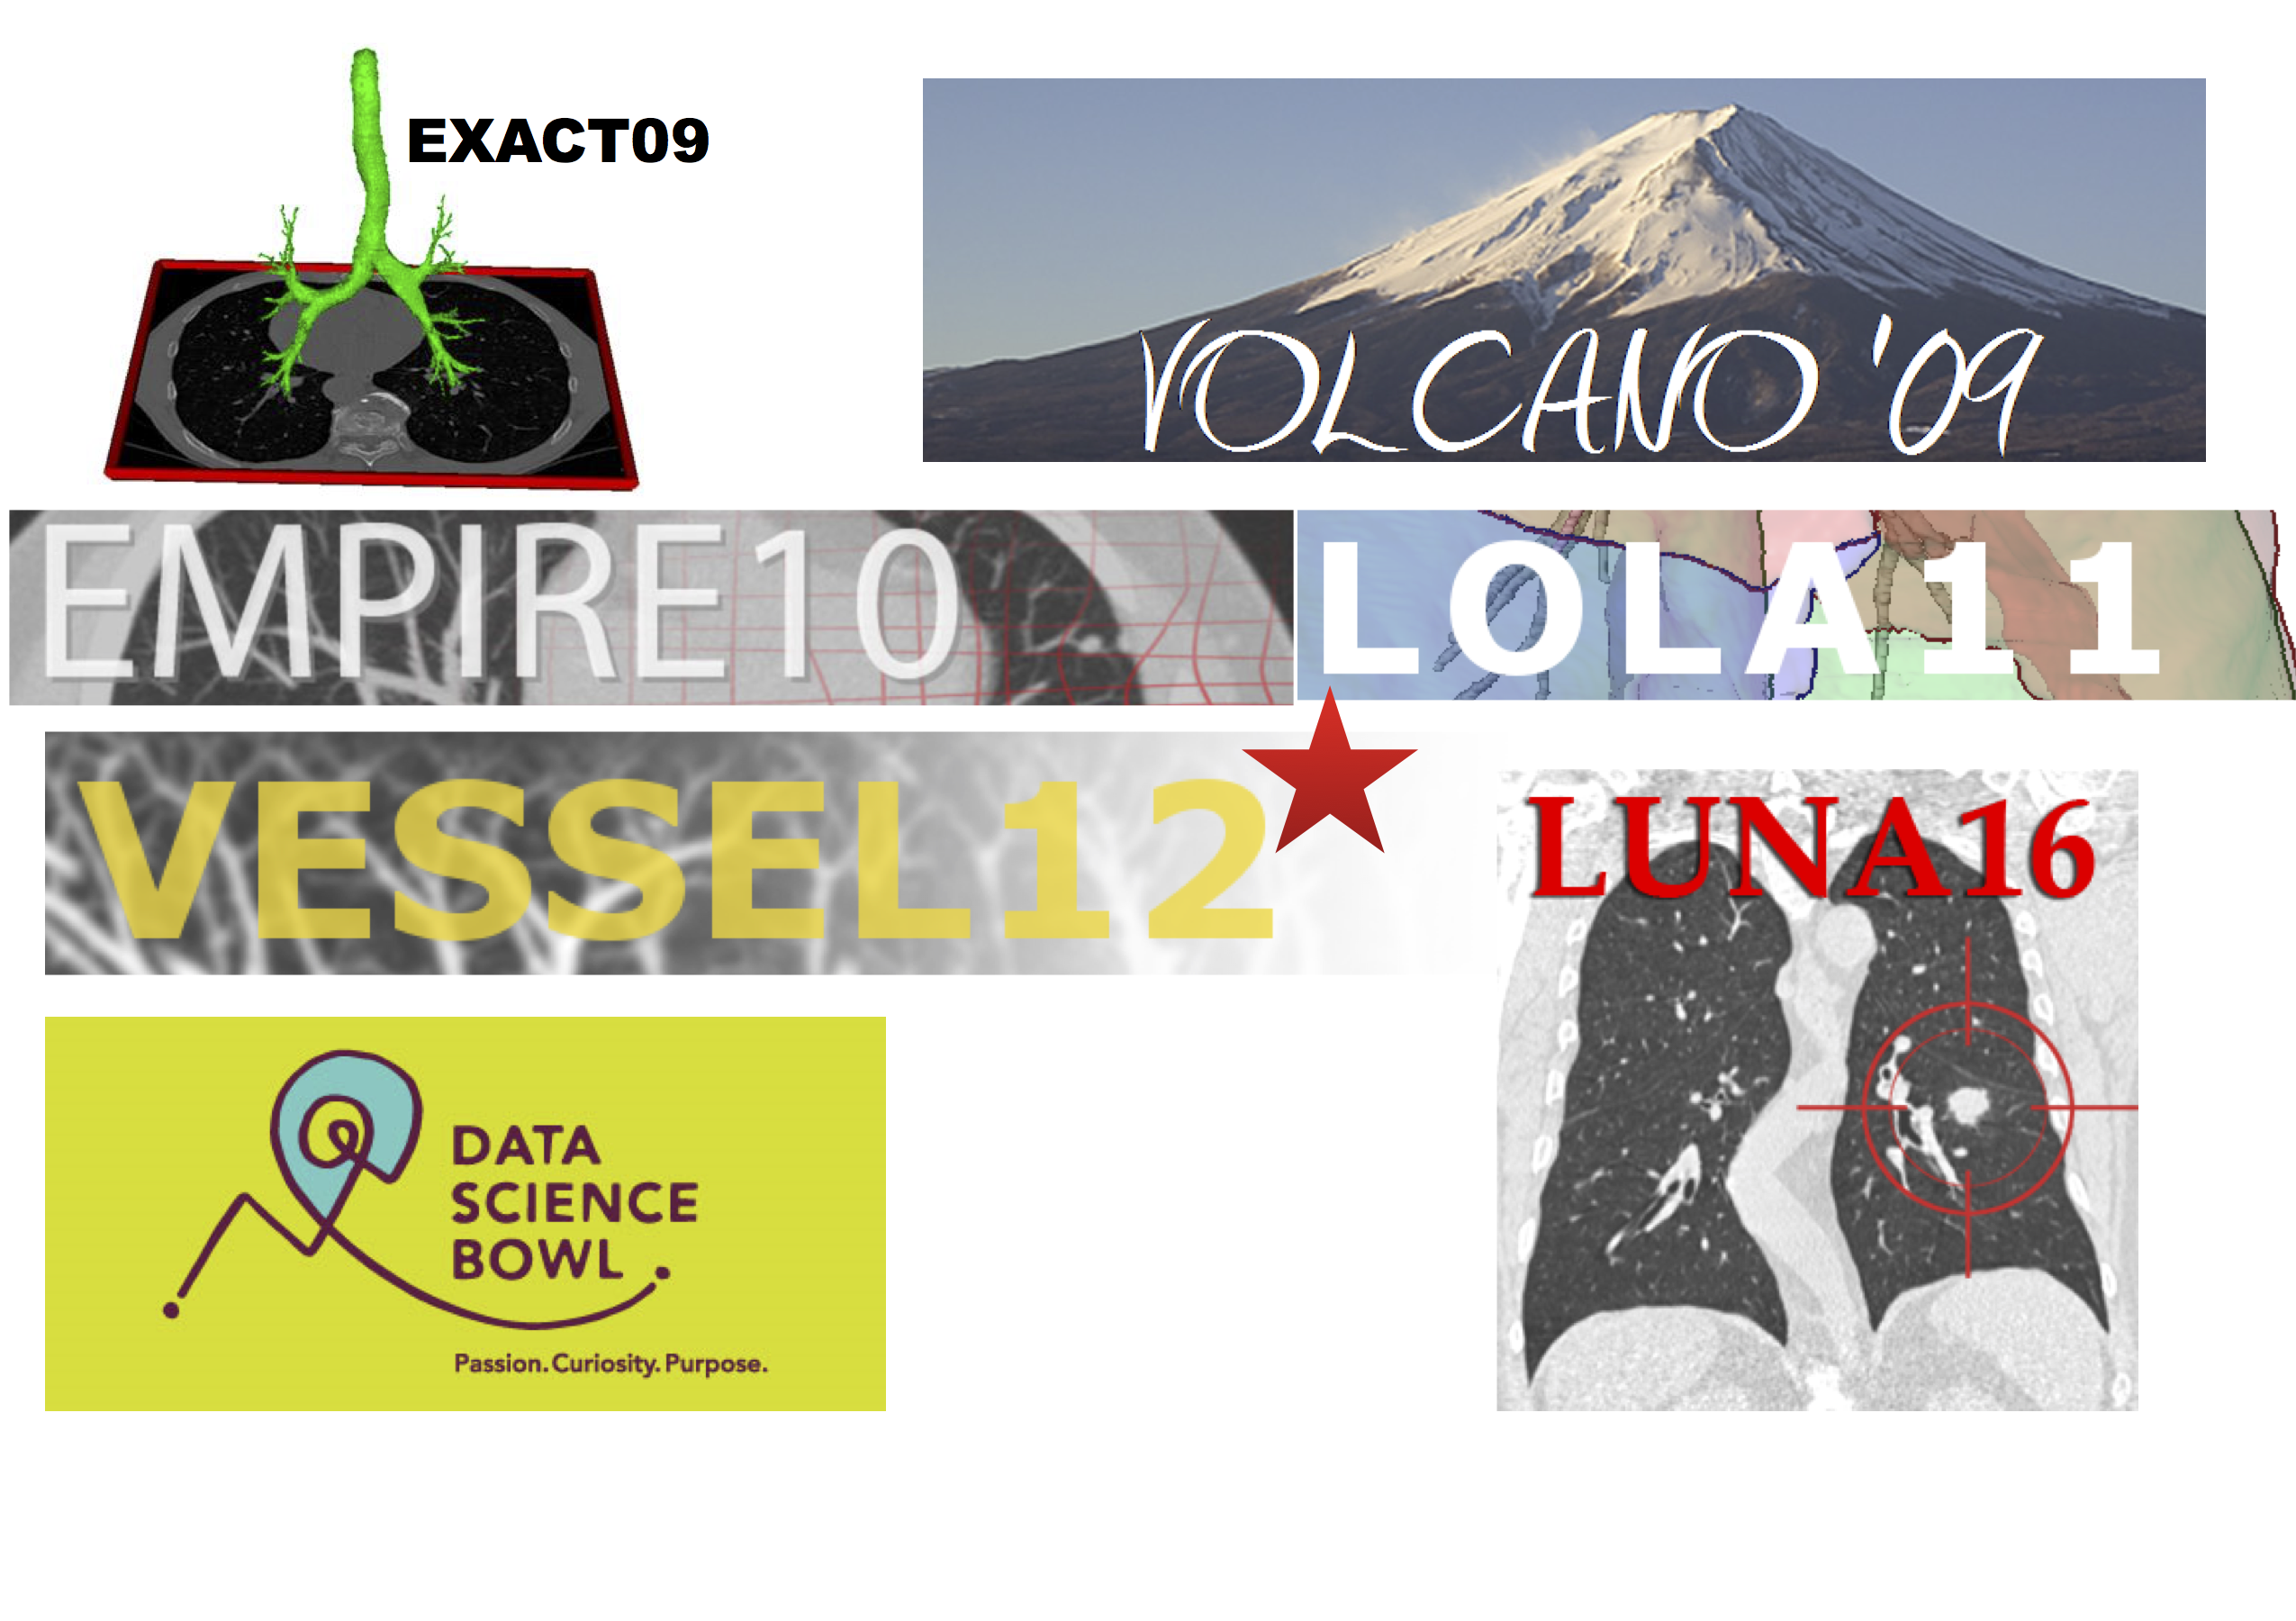
\includegraphics[width=0.95\textwidth]{./Figs/competitions.png}
\end{figure}

\end{frame}

\begin{frame}{What does the neuroimaging community offer?}

Great packages such as:

\begin{itemize}
\tightlist
\item
  AFNI
\item
  FSL
\item
  FreeSurfer \(\longrightarrow\)
  NeuroQuant\textsuperscript{\textregistered}
\item
  SPM
\item
  ANTs
\end{itemize}

\end{frame}

\begin{frame}{Public \& robust software \(\longrightarrow\) research
output}

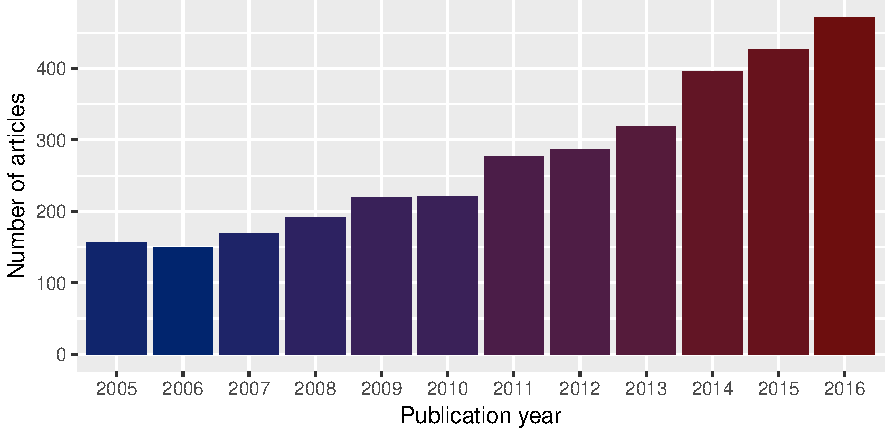
\includegraphics{stitchedIwpiSlides_files/figure-beamer/pubmedQuery-1.pdf}

\end{frame}

\begin{frame}{Benefits of open-source:}

\begin{itemize}
\tightlist
\item
  Motivates community-based support:

  \begin{itemize}
  \tightlist
  \item
    bug fixes (\emph{``Given enough eyeballs, all bugs are shallow.''}),
  \item
    new features,
  \item
    reproducibility, and
  \item
    community tech support.
  \end{itemize}
\item
  Learn directly from journal manuscripts \emph{and} implementations.
\item
  Tremendous cost-savings.
\item
  \emph{``Don't reinvent the wheel.''}
\end{itemize}

\end{frame}

\begin{frame}{ANTs core tools for neuroimage analysis}

\centering

\begin{figure}
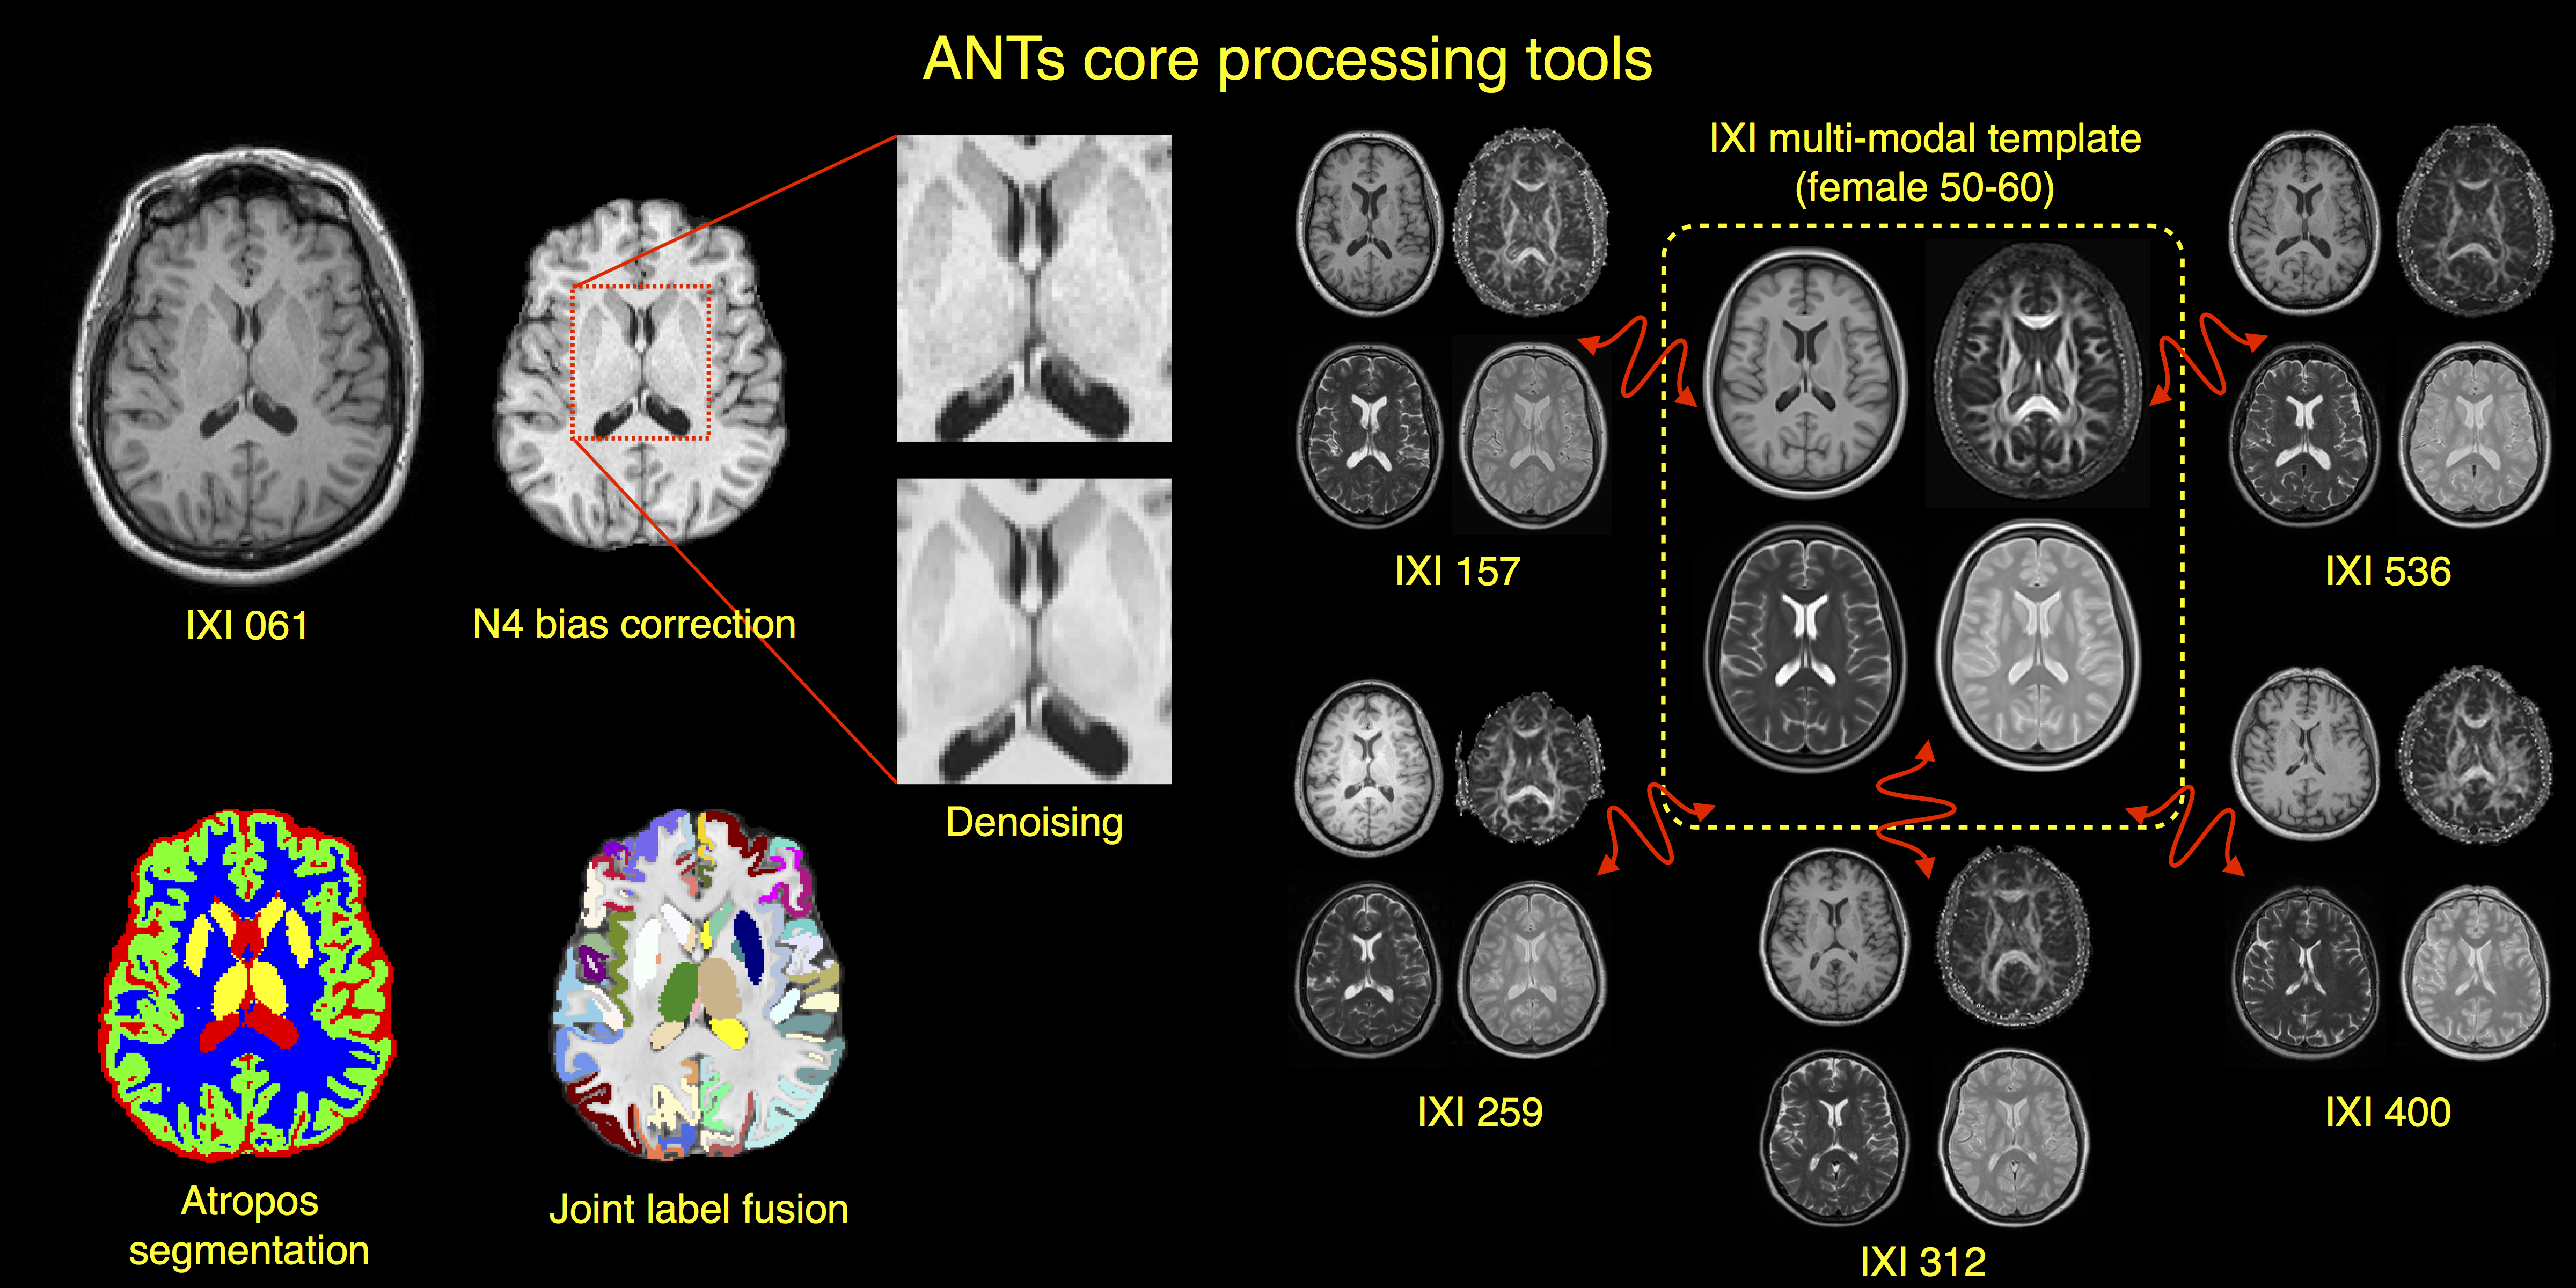
\includegraphics[width=0.95\textwidth]{../Figs/coreANtsToolsNeuro.png}
\end{figure}

\end{frame}

\section{ITK-Lung}\label{itk-lung}

\begin{frame}{ANTs core tools for lung image analysis}

\centering

\begin{figure}
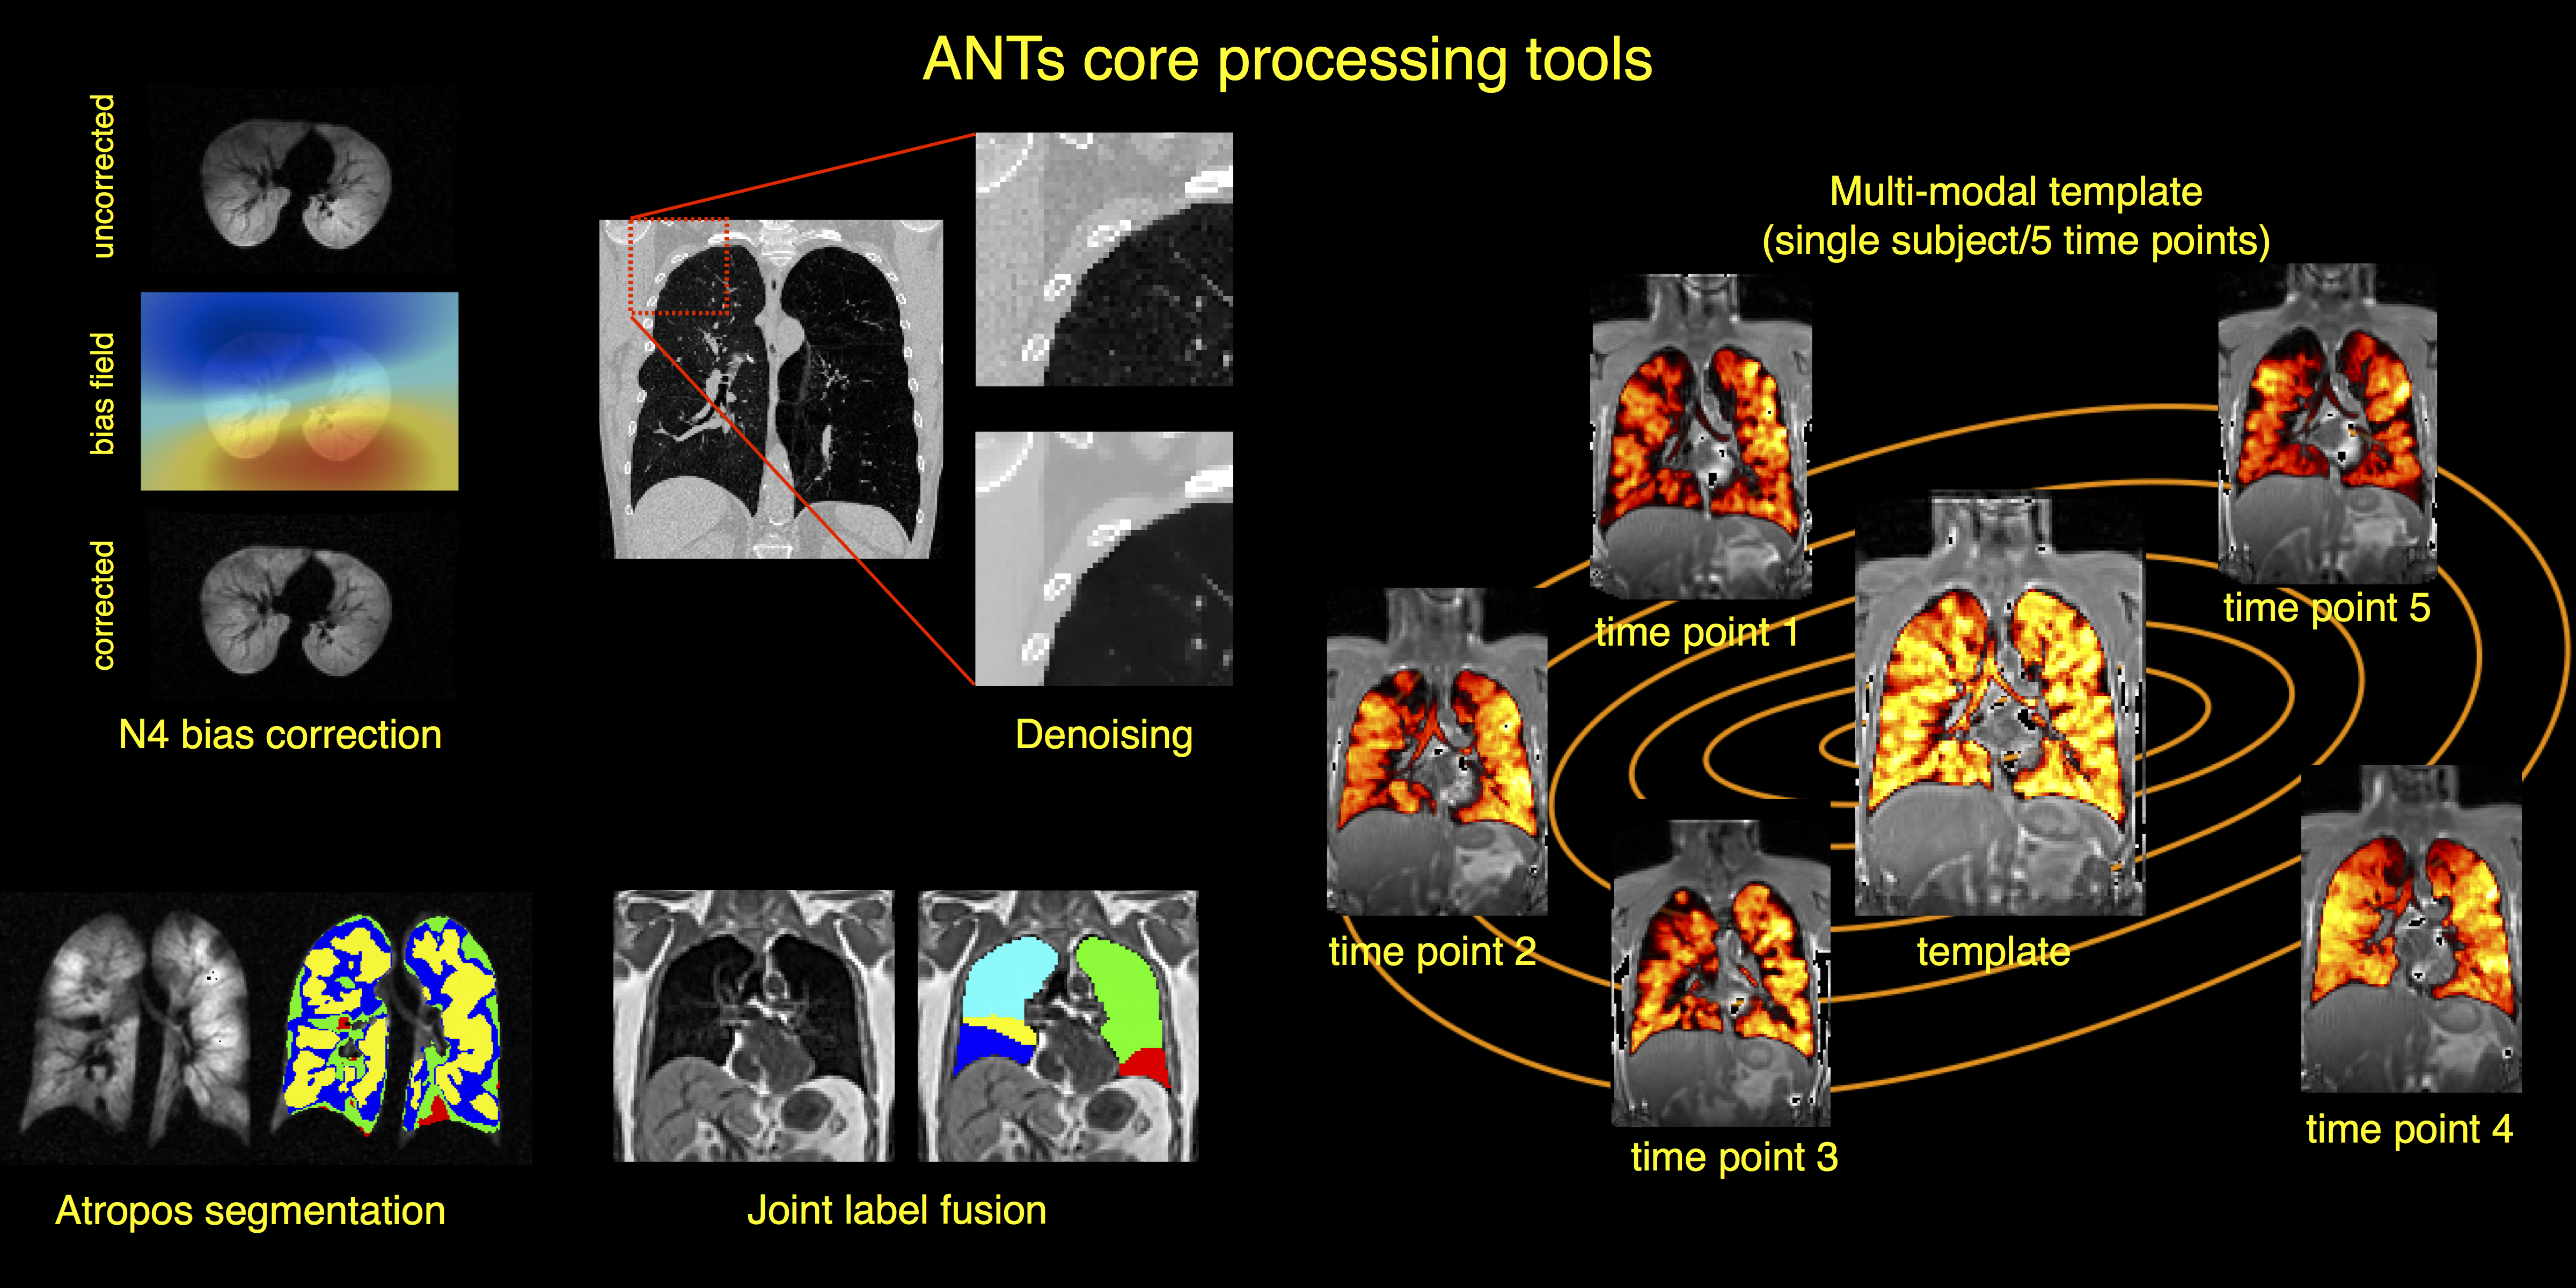
\includegraphics[width=0.95\textwidth]{./lung/figures/coreANtsToolsLung.png}
\end{figure}

\end{frame}

\begin{frame}{Proposed core functionality}

\begin{longtable}[c]{@{}lcccc@{}}
\toprule
\textbf{Functionality} & \textbf{CT} & \textbf{1H MRI} & \textbf{3He
MRI} & \textbf{PET}\tabularnewline
\midrule
\endhead
registration & \(\circ\) & \(\circ\) & \(\circ\) &
\(\circ\)\tabularnewline
template generation & \(\circ\) & \(\circ\) & \(\circ\) &
\(\circ\)\tabularnewline
lung segmentation & \(\circ\) & \(\circ\) & \(\ddagger\) &
\(\ddagger\)\tabularnewline
lobe segmentation & \(\circ\) & \(\circ\) & \(\ddagger\) &
\(\ddagger\)\tabularnewline
airway segmentation & \(\circ\) & -- & -- & --\tabularnewline
vessel segmentation & \(\circ\) & -- & -- & --\tabularnewline
functional segmentation & \(\ast\) & -- & \(\circ\) &
\(\ast\)\tabularnewline
feature indices & \(\circ\) & -- & \(\ast\) & \(\ast\)\tabularnewline
\bottomrule
\end{longtable}

\footnotesize

'\(\circ\)': previously published work

'\(\ast\)': cross-modality functionality

'\(\ddagger\)': simultaneous structural acquisitions

\hypertarget{refs}{}

\end{frame}

\end{document}